\documentclass{article}

\usepackage{polski}
\usepackage[utf8]{inputenc}

%Check documentation
\usepackage{fancyhdr}
\usepackage{graphicx}
\pagestyle{fancy}
\fancyhead{}
\fancyfoot{}
\fancyfoot[R]{\thepage}
\renewcommand{\headrulewidth}{0pt}
\renewcommand{\footrulewidth}{0pt}

\usepackage{lipsum}

\begin{document}
\begin{titlepage}
	\begin{center}
		\textsc{\LARGE Politechnika Śląska}\\
		[1cm]
		\textsc{\large Wydział Matematyki Stosowanej}\\
		[0.5cm]
		\textsc{\normalsize Projekt z Informatyki}\\
		\line(1,0){300}\\
		[0.2cm]
		\textbf{\LARGE Szyfrowanie Wiadomości}\\	
		[0.3cm]
		\line(1,0){300}\\
		[2cm]
	\end{center}
	
	\begin{flushright}
		\textbf{Student: }\\
		\textsc{Kamil Król}
	\end{flushright}
	
	\vspace{\fill}
	\begin{center}
		\textsc{2 Stycznia, 2018}
	\end{center}
	
\end{titlepage} 

\tableofcontents
\thispagestyle{empty}
\cleardoublepage

\setcounter{page}{1}

\section{Opis programu}\label{sec:intro}
Projekt jest rozwiązaniem zadania z konkursu Algorytmion 2015 - zadanie1 - "SZYFROWANIE WIADOMOŚCI".

Program ma za zadanie zaszyfrować wiadomość z pliku a następnie odszyfrować podaną wiadomość.\\

\textsc{\large Opis szyfru:}

\begin{itemize}
\item Każdą literę i znak interpunkcyjny należy zamienić na odpowiadającą liczbę kodu ASCII(liczba naturalna od 0 do 127).
\item Pierwsza, tak powstała liczba, jest zamieniana na system dwójkowy.
\item Kolejne liczby, wynikające z kodu ASCII, są zamieniane na system liczbowy, który jest równy powiększonej o dwa reszcie z dzielenia przez osiem poprzedniej liczby.
\item Ilość cyfr zamienionej liczby, dla każdego systemu liczbowego, wynika z ilości cyfr
zamiany liczby maksymalnej, czyli liczby 127 (dla systemu binarnego jest to siedem
cyfr).
\end{itemize}

\textsc{\large Kolejność wykkonywanych działań programu:}
\begin{itemize}
\item Pobranie wiadomości z pliku text.txt (tylko pierwsza linijka)
\item Szyfrowanie wiadomości
\item Przesłanie kryptogramu do pliku szyfr.txt
\item Odczyt kryptogramu z pliku szyfr.txt
\item Odszyfrowanie wiadomości
\item Wysłanie odszyfrowanej wiadomości do pliku odszyfrowane.txt
\end{itemize}


\newpage

\section{Instrukcja Obsługi}
Do poprawnego działania programu wymagane jest utworzenie pliku szyfr.txt w folderze zawierającym program("projekt").

Do pliku szyfr.txt należy wprowadzić tylko jedną linijkę tekstu który życzymy sobie zaszyfrować.

Następnie należy uruchomić program który wyświetli w konsoli tylko jedą wiadomość:\\

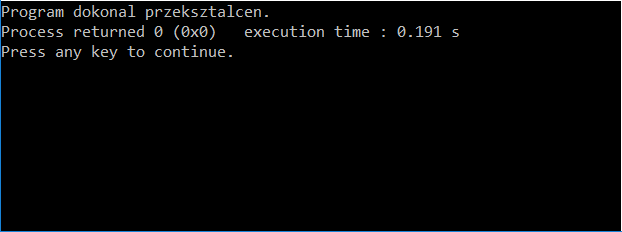
\includegraphics{message}\\

Po zakończeniu działania programu zaszyfrowana wiadomośc pojawi sie w pliku szyfr.txt, zaś odszyfrowana w pliku odszyfrowanie.txt.

\cleardoublepage

\section{Techniczny Opis Programu}

Program został napisany w języku C++ za pomocą IDE Code::Blocks oraz kompilatora GNU GCC Compiler.

\subsection{Biblioteki}
Do poprawnego działania programu zostaly użyte trzy biblioteki.

\begin{itemize}
\item iostream - w celu wypisania wiadomości
\item fstream - w celu możliwości pracy na plikach
\item string - w celu wykorzystania funkcji dzialających na ciągach znaków takich jak length()
\end{itemize}

\subsection{Funkcja main()}
Funkcja main ma za zadanie odczyt danych z plików oraz wywołanie funkcji pomocniczych do szyfrowania jak i odszyfrowania wiadomości.

\subsection{Funkcje pomocnicze}
\textsc{\large Funkcje szyfrujące:}

\begin{itemize}
\item void szyfrowanie(string dane)

funkcja szyfruje podany ciąg znaków oraz przesyła kryptogram do pliku
\item string usuniecie\_spacji(string dane)

funkcja usuwa spacje z podanego ciągu
\item string zamiana\_systemu(char znak, int system)

funckja zamienia pojedynczy znak tekstu na szyfr w podanym systemie liczbowym
\end{itemize}


\textsc{\large Funkcje deszyfrujące:}

\begin{itemize}
\item void odszyfrowywanie(string dane)

funckja odszyfrowuje dany ciag znaków i wysyła go do pliku
\item char odszyfrowanie\_znaku(string znak, int system)

funkcja odszyfrowuje pojedynczy znak
\end{itemize}

\cleardoublepage

\section{Szczegóły techniczne}

Szyfrowanie danych polega na algorytmie symetrycznym, gdyż ten sam algorytm co szyfruje dane jest wykorzystywany do ich odszyfrowania.\\

Przykładowe szyfrowanie wiadomości "Ola".\\

\begin{tabular}{|l|l|l|l|} \hline
Znak & ASCII & System & Szyfr\\
\hline \hline
O & 79 & 2 & 1001111\\
\hline \hline
l & 108 & (79mod8)+2=9 & 130\\ \hline
\hline \hline
a & 97 & (108mod8)+2=6 & 241\\ \hline
\end{tabular}\\

"O" posiada numer 79 w ASCII pierwszy znak szyfrujemy za pomocą systemu dwójkowego zatem $79_{(2)}$ = 1001111.\\

"l" posiada numer 108 w ASCII.
Żeby obliczyć kolejny system liczbowy do zaszyfrowania wykonujemy działanie (wczesniejszy znak(nr.ASCII) mod 8)+2 = system.\\
Zatem (79mod8)+2=9.\\
Teraz szyfrujemy znak za pomocą uzyskanego systemu liczbowego.
$108_{(9)}$ = 130.\\\\
Tak samo postępujemy z kolejnymi znakami aż do ich wyczerpania.\\


Stosując powyższy algorytm dla słowa "Ola" uzyskamy szyfr w postaci:
\begin{center}
1001111 130 241\\
\end{center}

Odszyfrowywanie wyglada bardzo podobnie co szyfrowanie:\\

\begin{tabular}{|l|l|l|l|} \hline
Szyfr & System & ASCII(dziesiętny) & Znak\\
\hline \hline
1001111 & 2 & 79 & O\\
\hline \hline
130 & (79mod8)+2=9 & 108 & l\\ \hline
\hline \hline
241 & (108mod8)+2=6 & 97 & a\\ \hline
\end{tabular}\\

Wiemy, że pierwszy znak jest zaszyfrowany w systemie dwójkowym zatem.\\
$1001111_{(2)}$ = $79_{(10)}$.\\
Numer 79 w ASCII oznacza znak "O"

Żeby poznać w jakim systemie został zaszyfrowany kolejny znak stosujemy ten sam wzór co do szyfrowania:\\\\
(wczesniejszy znak(nr.ASCII) mod 8)+2 = system.\\

Zatem (79mod8)+2=9.\\
Po otrzymaniu systemu odszyfrowujemy znak.
$130_{(9)}$ = $108_{(10)}$\\
Numer 108 w ASCII oznacza znak "l"

Tak samo postępujemy z kolejnymi zaszyfrowanymi znakami aż do ich wyczrpania.
\end{document}